\chapter{Конструкторская часть}

В данном разделе будет рассмотрена схема алгоритма нахождения обратной матрицы методом Гаусса-Жордана
и его версия параллельная версия.

\section{Требование к прогаммному обеспечению}

К программе предъявляются следующие требования:

\begin{itemize}
	\item на вход подается размерность матрицы, элементы матрицы;
	\item на выходе —-- матрица, обратная данной.
\end{itemize}

\section{Разработка алгоритмов}

На рисунках \ref{fig:gauss1}-\ref{fig:gauss2} представлена схема алгоритма
метода Гаусса-Жордана для нахождения обратной матрицы, на рисунках
\ref{fig:paral1}-\ref{fig:paral5} -- схема параллельного алгоритма.
На рисунках \ref{fig:mult}-\ref{fig:swap} представлены вспомогательные функции.

\begin{figure}[h]
    \centering
    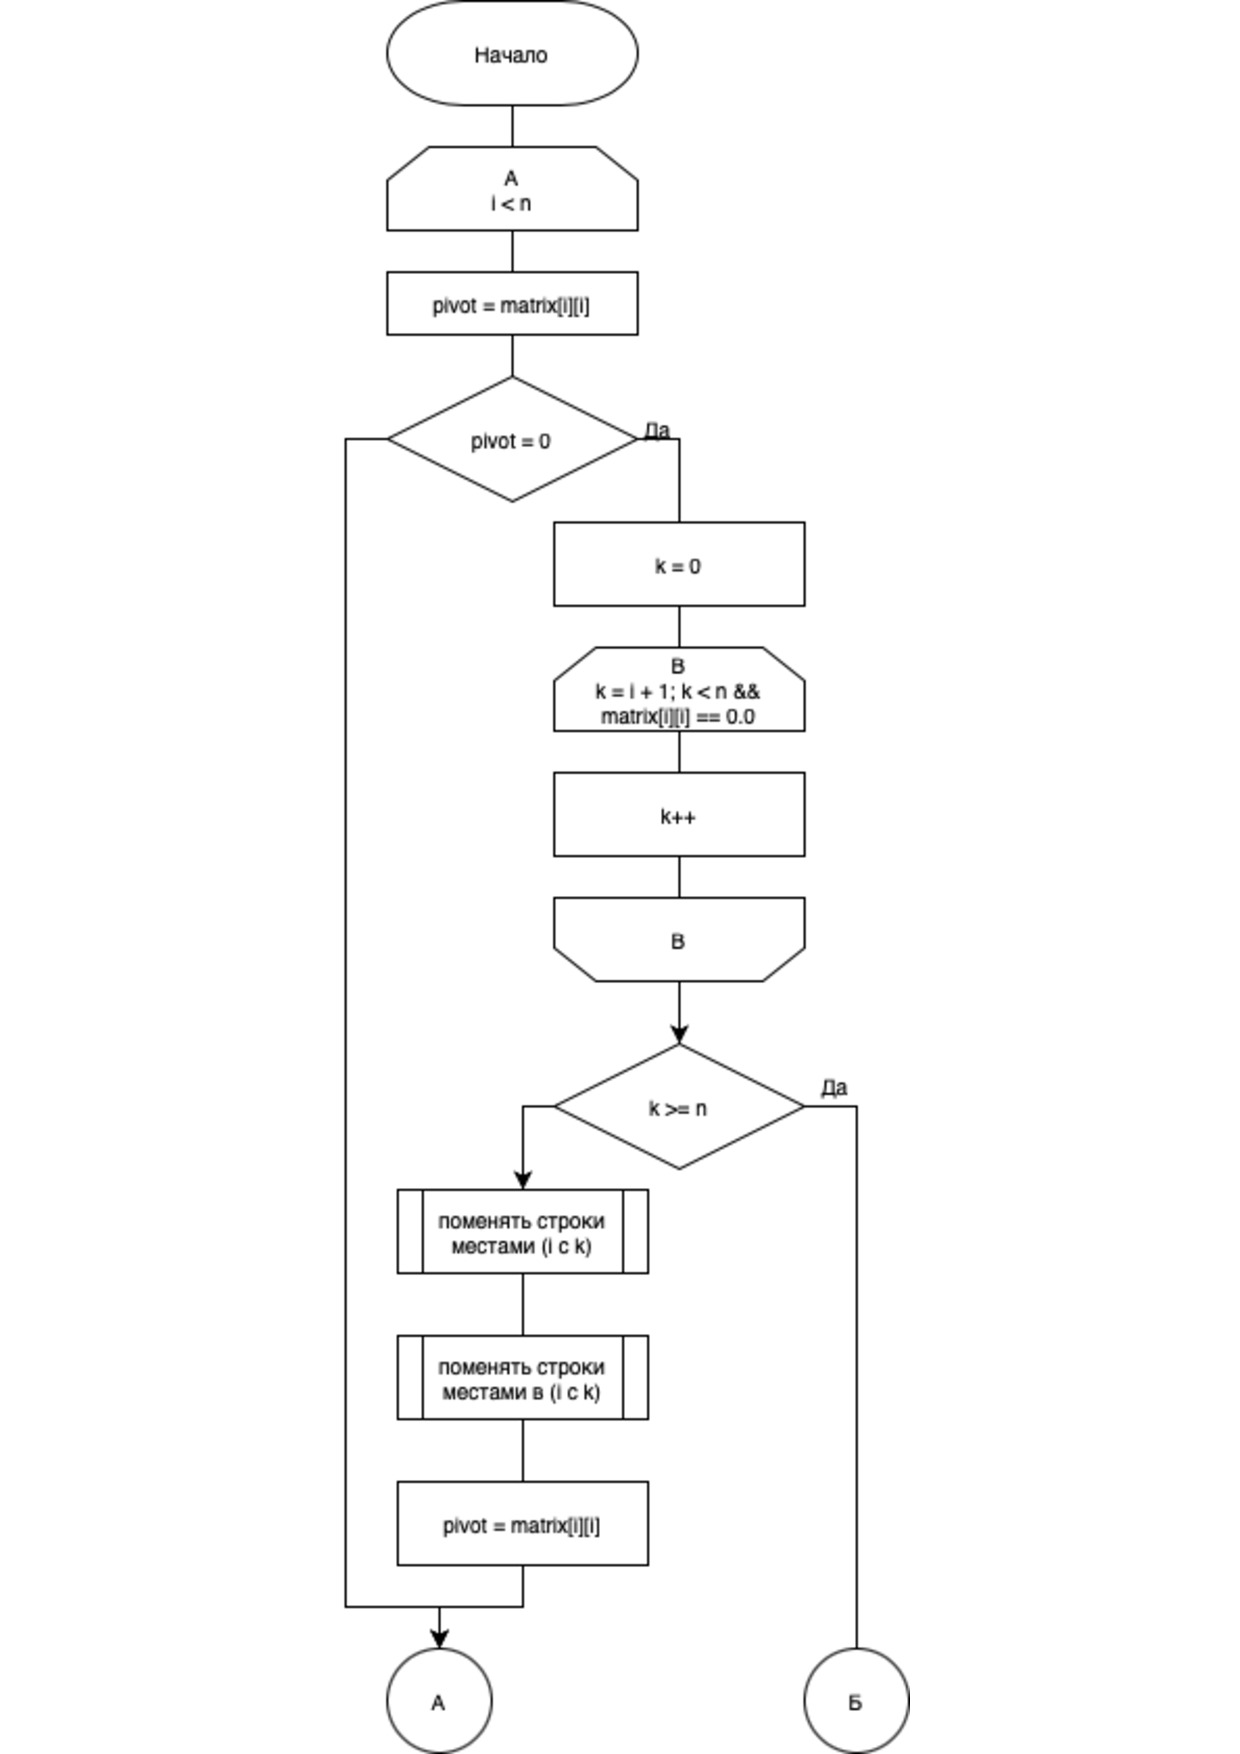
\includegraphics[width=0.9\linewidth]{img/gauss1.pdf}
    \caption{Схема алгоритма основной функции метода Гаусса-Жордана}
    \label{fig:gauss1}
\end{figure}

\begin{figure}[h]
    \centering
    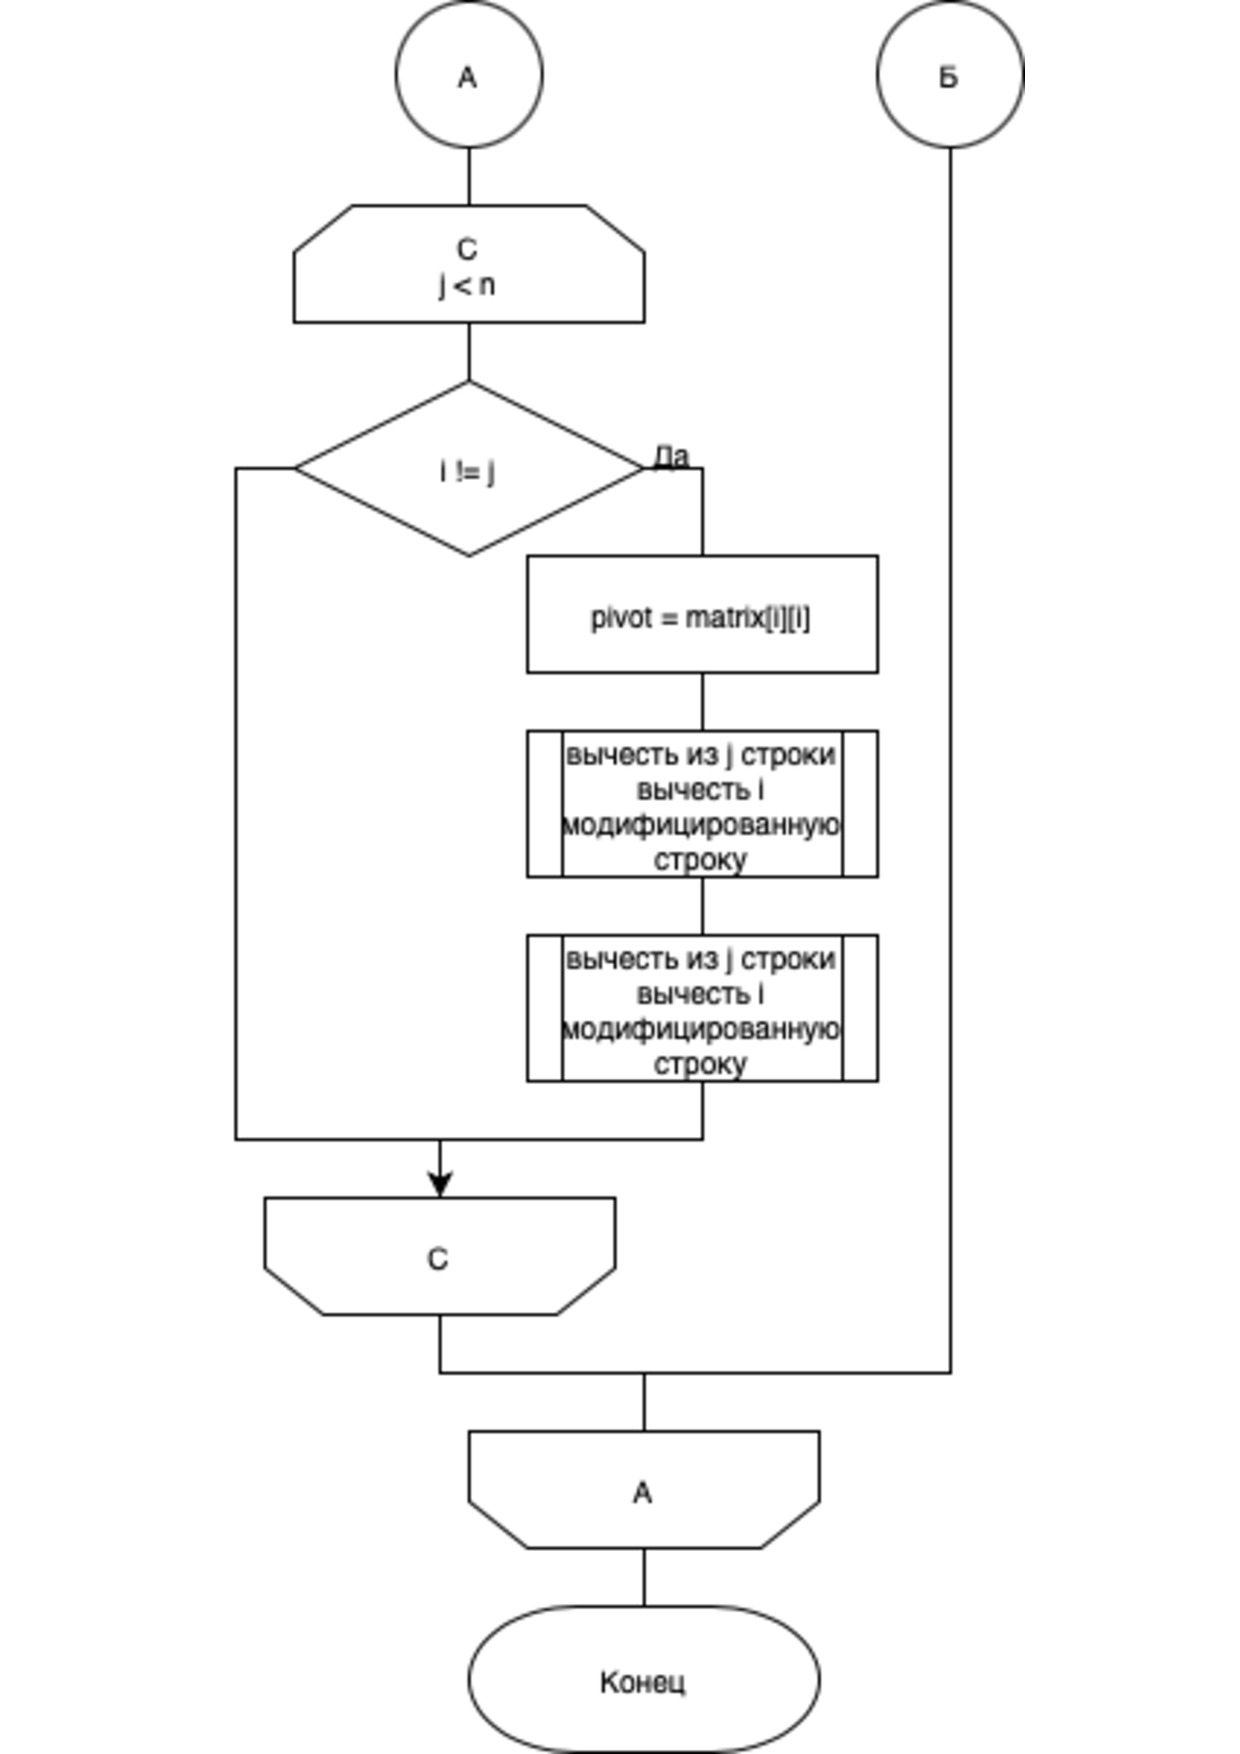
\includegraphics[width=0.7\linewidth]{img/gauss2.pdf}
    \caption{Схема алгоритма основной функции метода Гаусса-Жордана}
    \label{fig:gauss2}
\end{figure}

\begin{figure}[h]
    \centering
    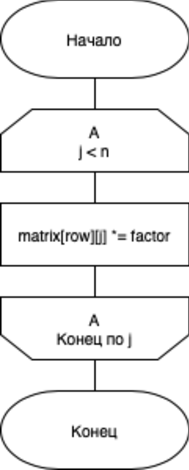
\includegraphics[width=0.25\linewidth]{img/mult.pdf}
    \caption{Схема алгоритма умножения строки матрицы на элемент}
    \label{fig:mult}
\end{figure}

\begin{figure}[h]
    \centering
    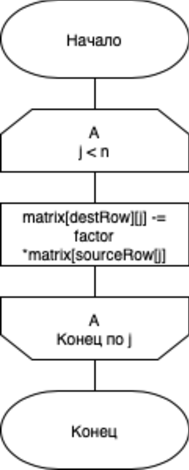
\includegraphics[width=0.25\linewidth]{img/submult.pdf}
    \caption{Схема алгоритма вычитания из строк матрицы модифицированной текущей строки}
    \label{fig:submult}
\end{figure}

\begin{figure}[h]
    \centering
    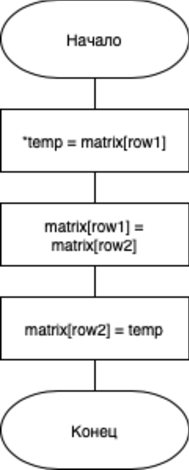
\includegraphics[width=0.25\linewidth]{img/swap.pdf}
    \caption{Схема алгоритма смены строк местами}
    \label{fig:swap}
\end{figure}

\begin{figure}[h]
    \centering
    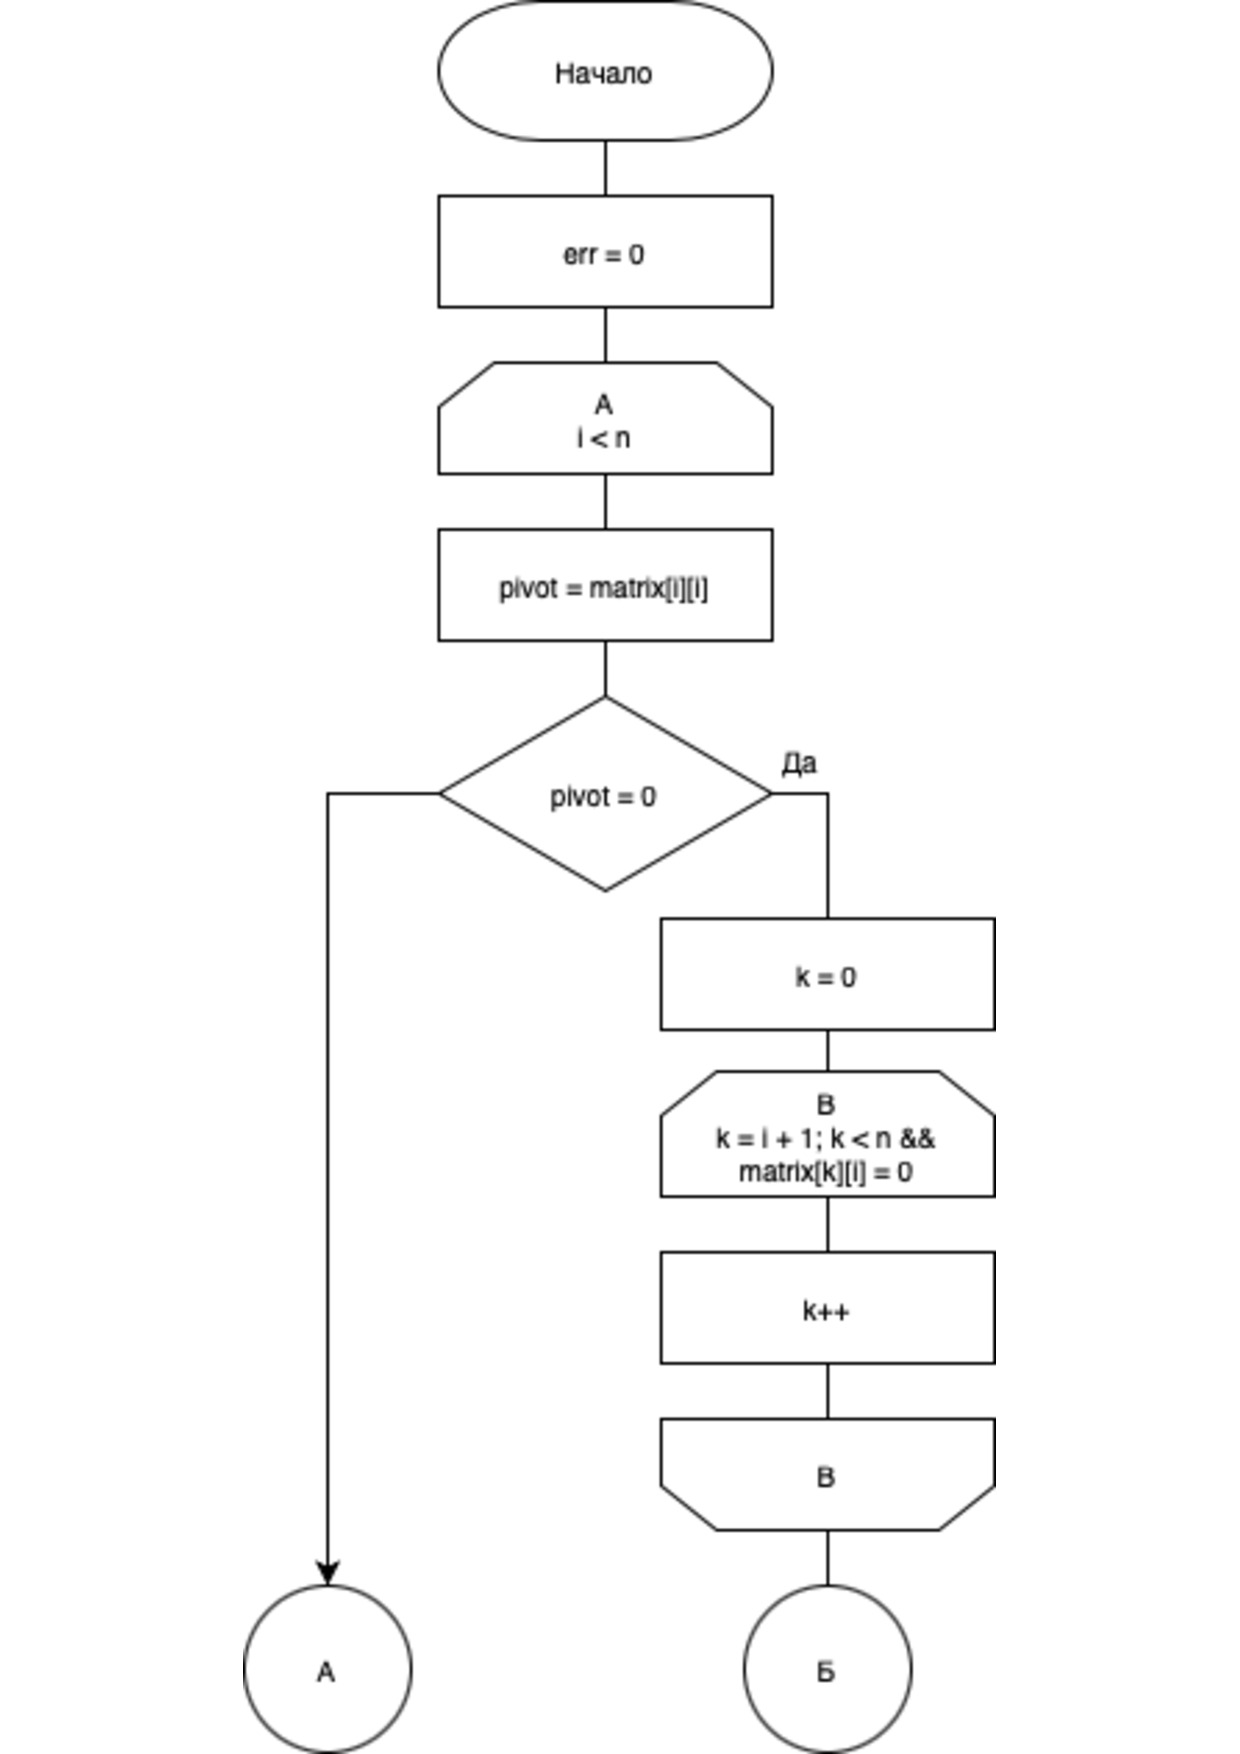
\includegraphics[width=0.7\linewidth]{img/paral1.pdf}
    \caption{Схема параллельного алгоритма основной функции метода Гаусса-Жордана}
    \label{fig:paral1}
\end{figure}

\begin{figure}[h]
    \centering
    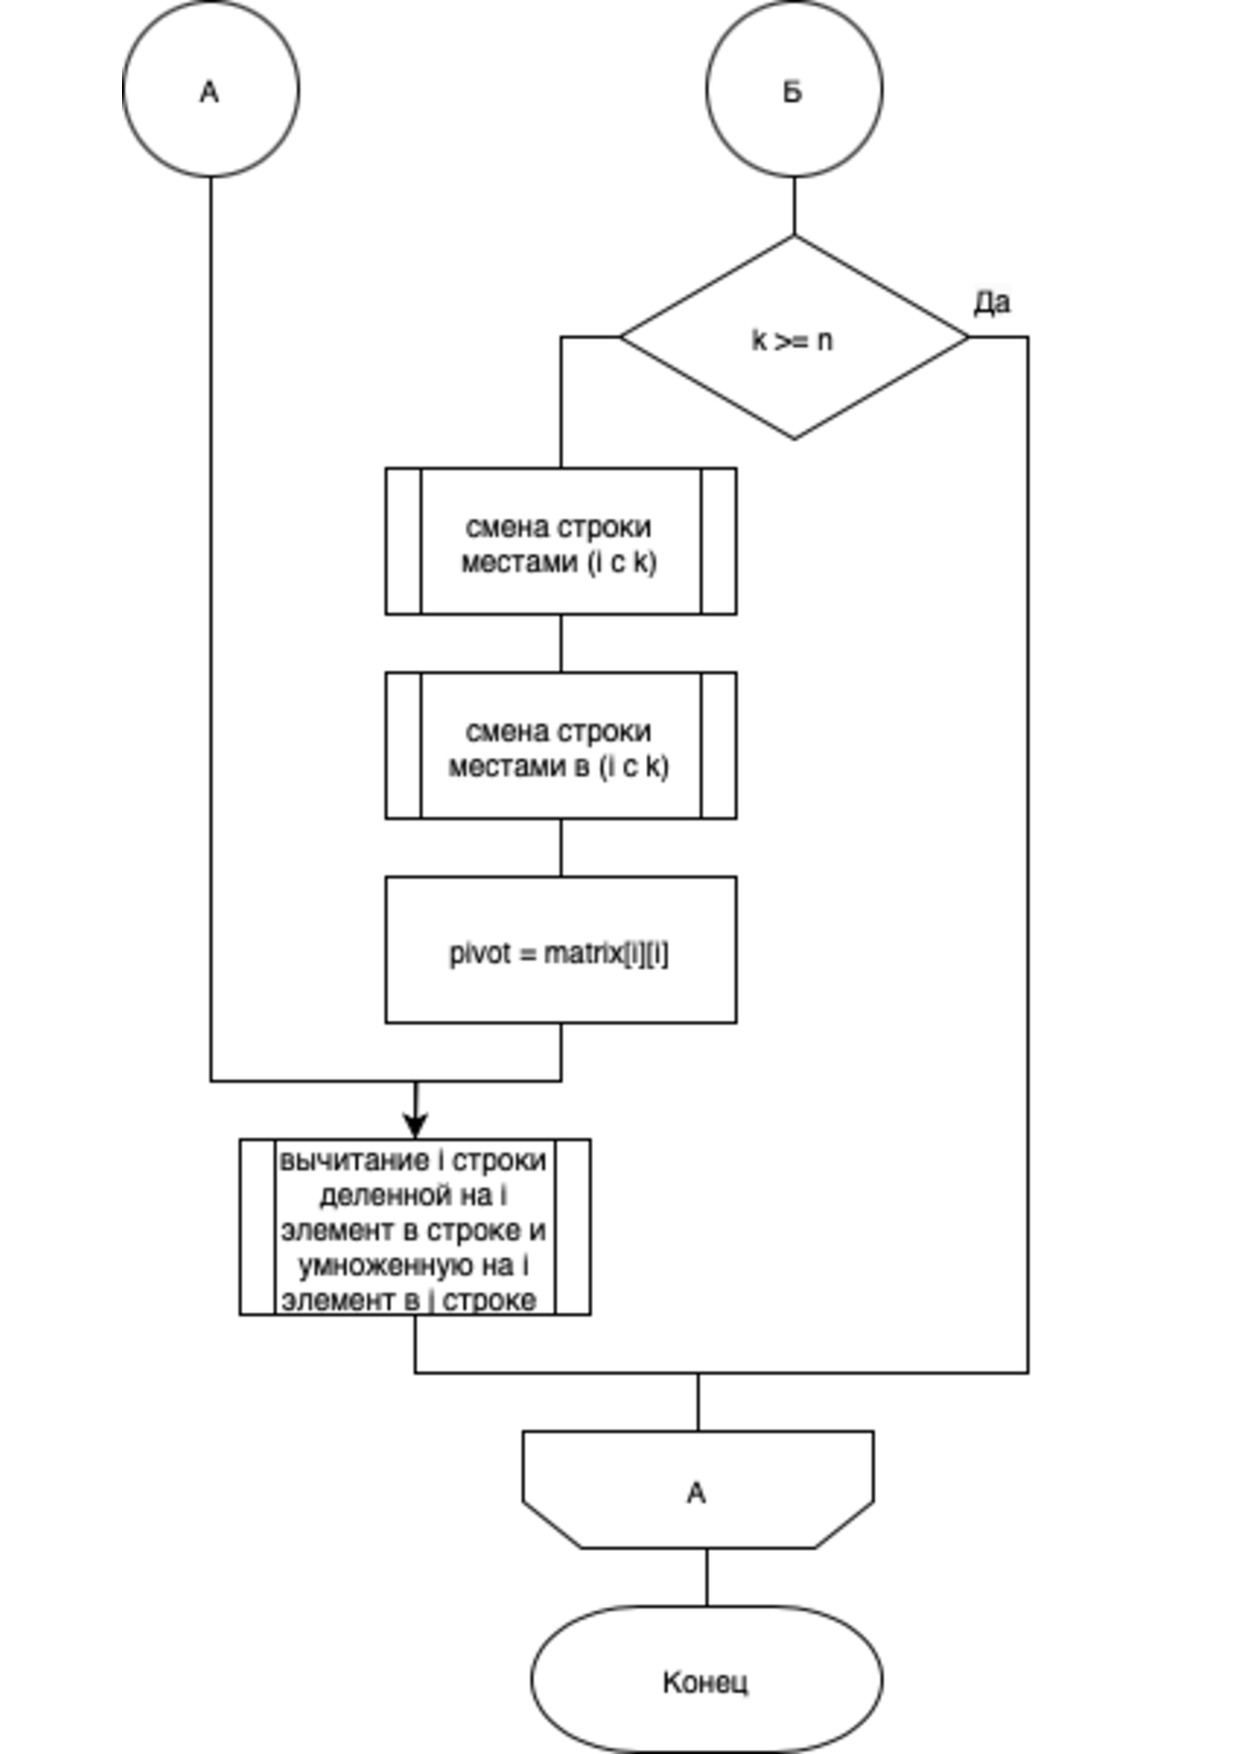
\includegraphics[width=0.7\linewidth]{img/paral2.pdf}
    \caption{Схема параллельного алгоритма основной функции метода Гаусса-Жордана}
    \label{fig:paral2}
\end{figure}

\begin{figure}[h]
    \centering
    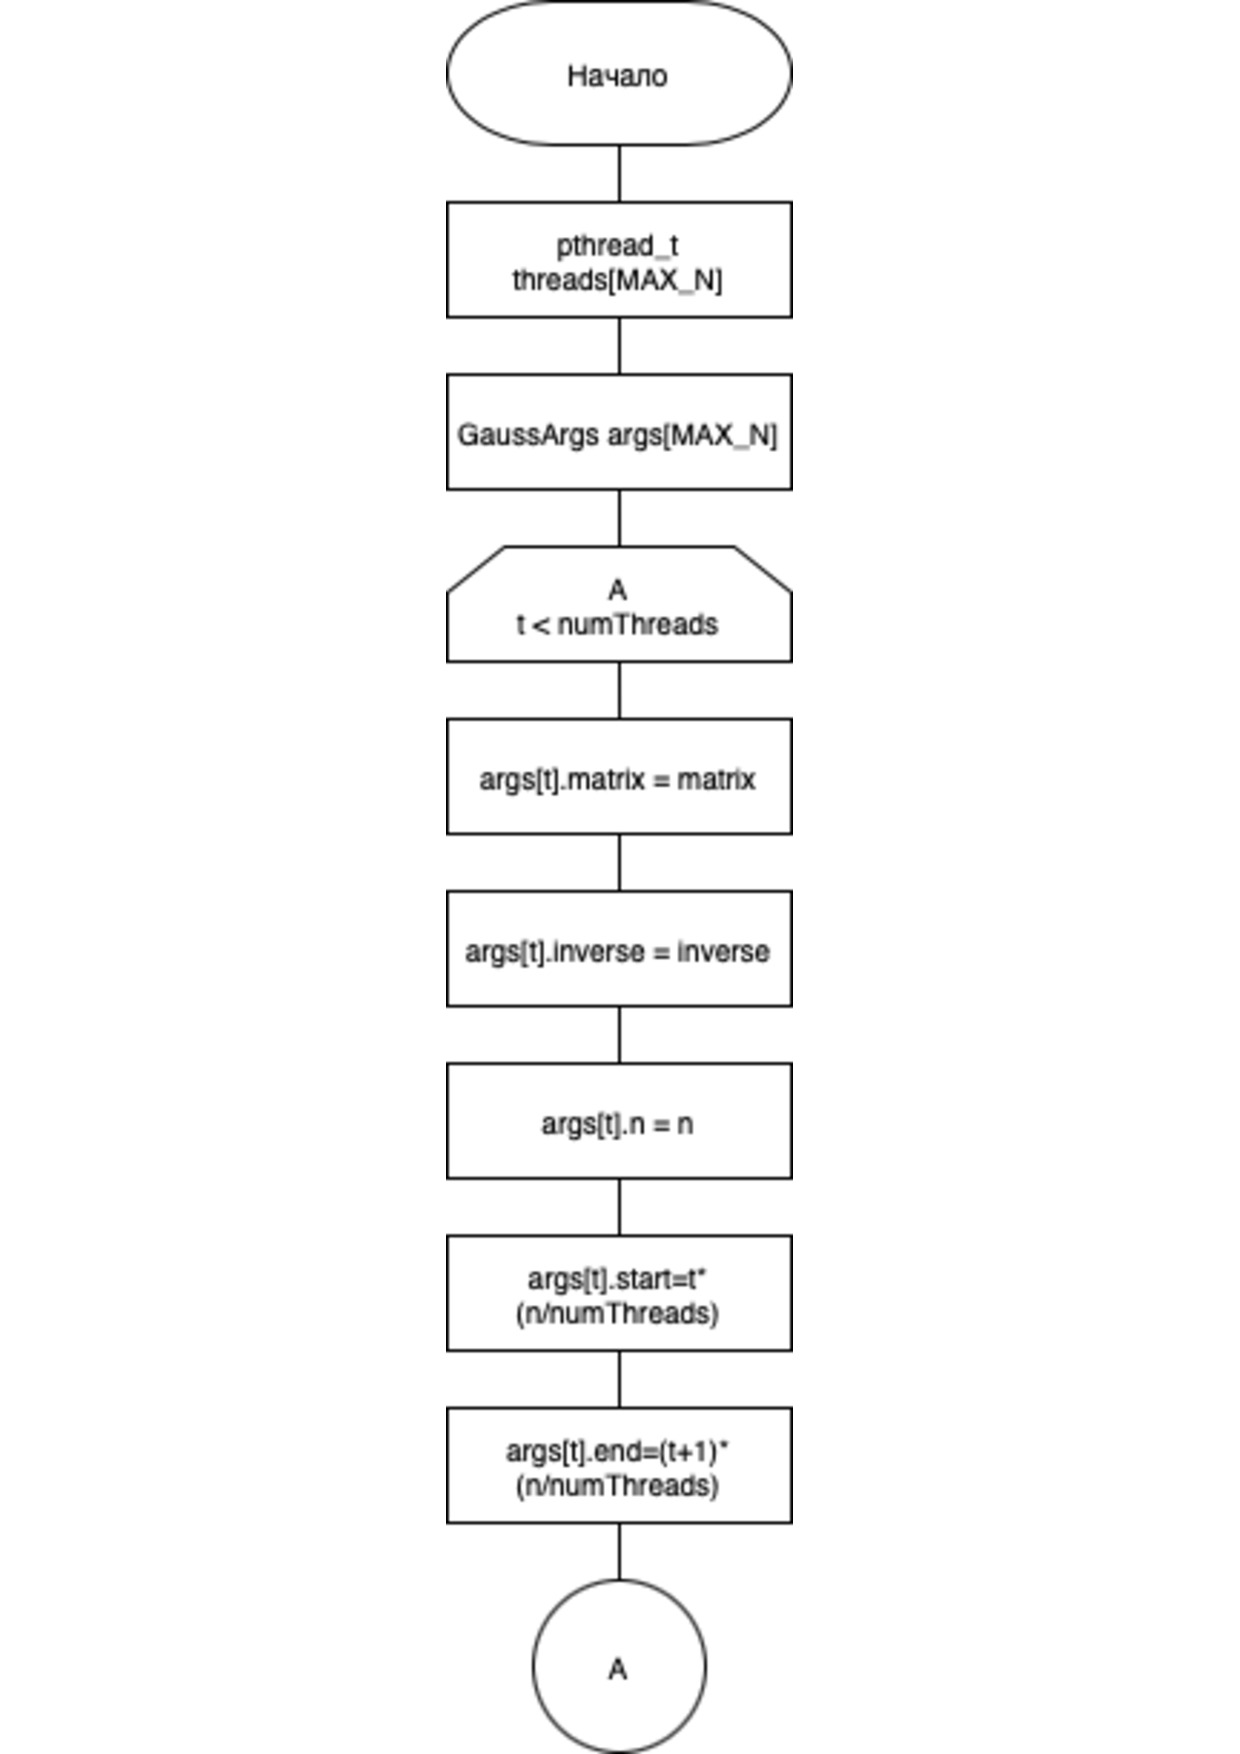
\includegraphics[width=0.75\linewidth]{img/paral3.pdf}
    \caption{Схема функции алгоритма, где происходит распараллеливание}
    \label{fig:paral3}
\end{figure}

\begin{figure}[h]
    \centering
    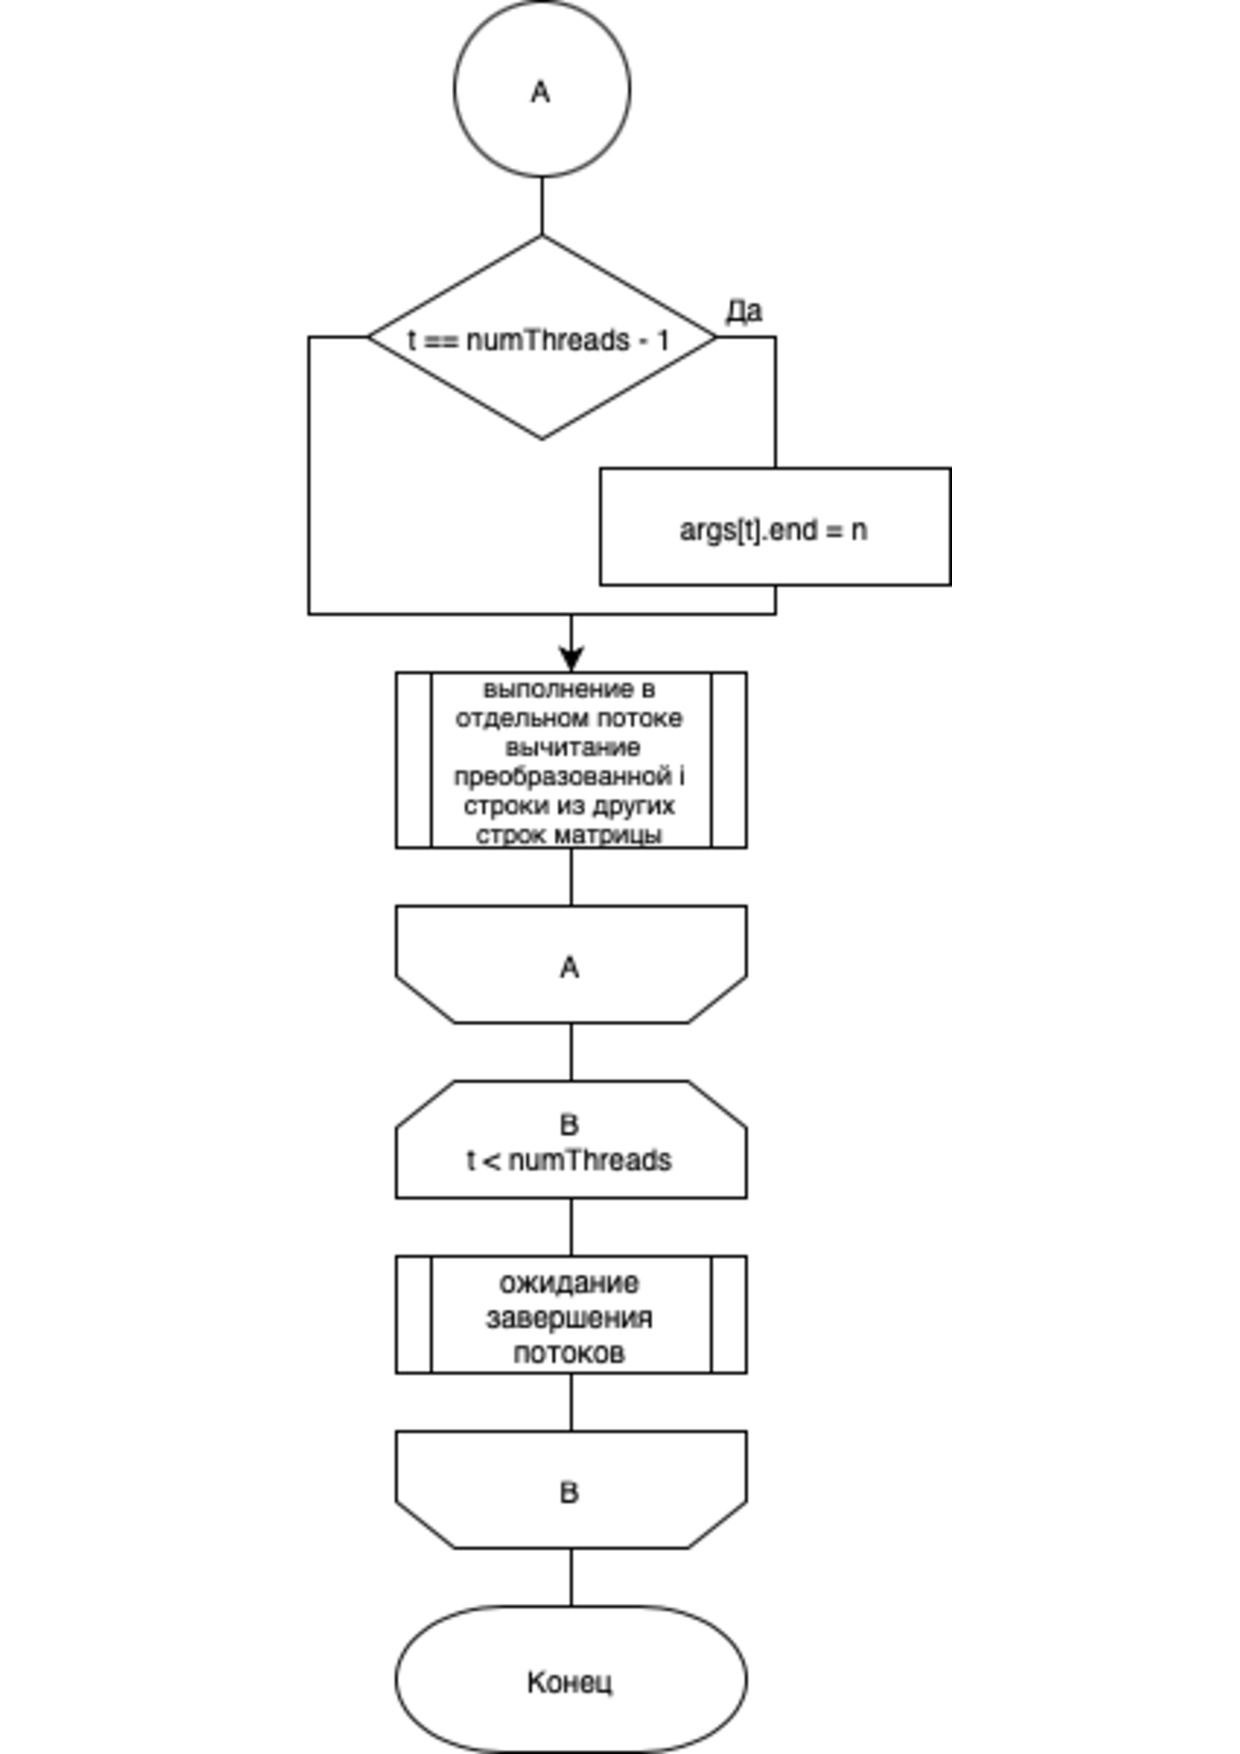
\includegraphics[width=0.7\linewidth]{img/paral4.pdf}
    \caption{Схема функции алгоритма, где происходит распараллеливание}
    \label{fig:paral4}
\end{figure}

\begin{figure}[h]
    \centering
    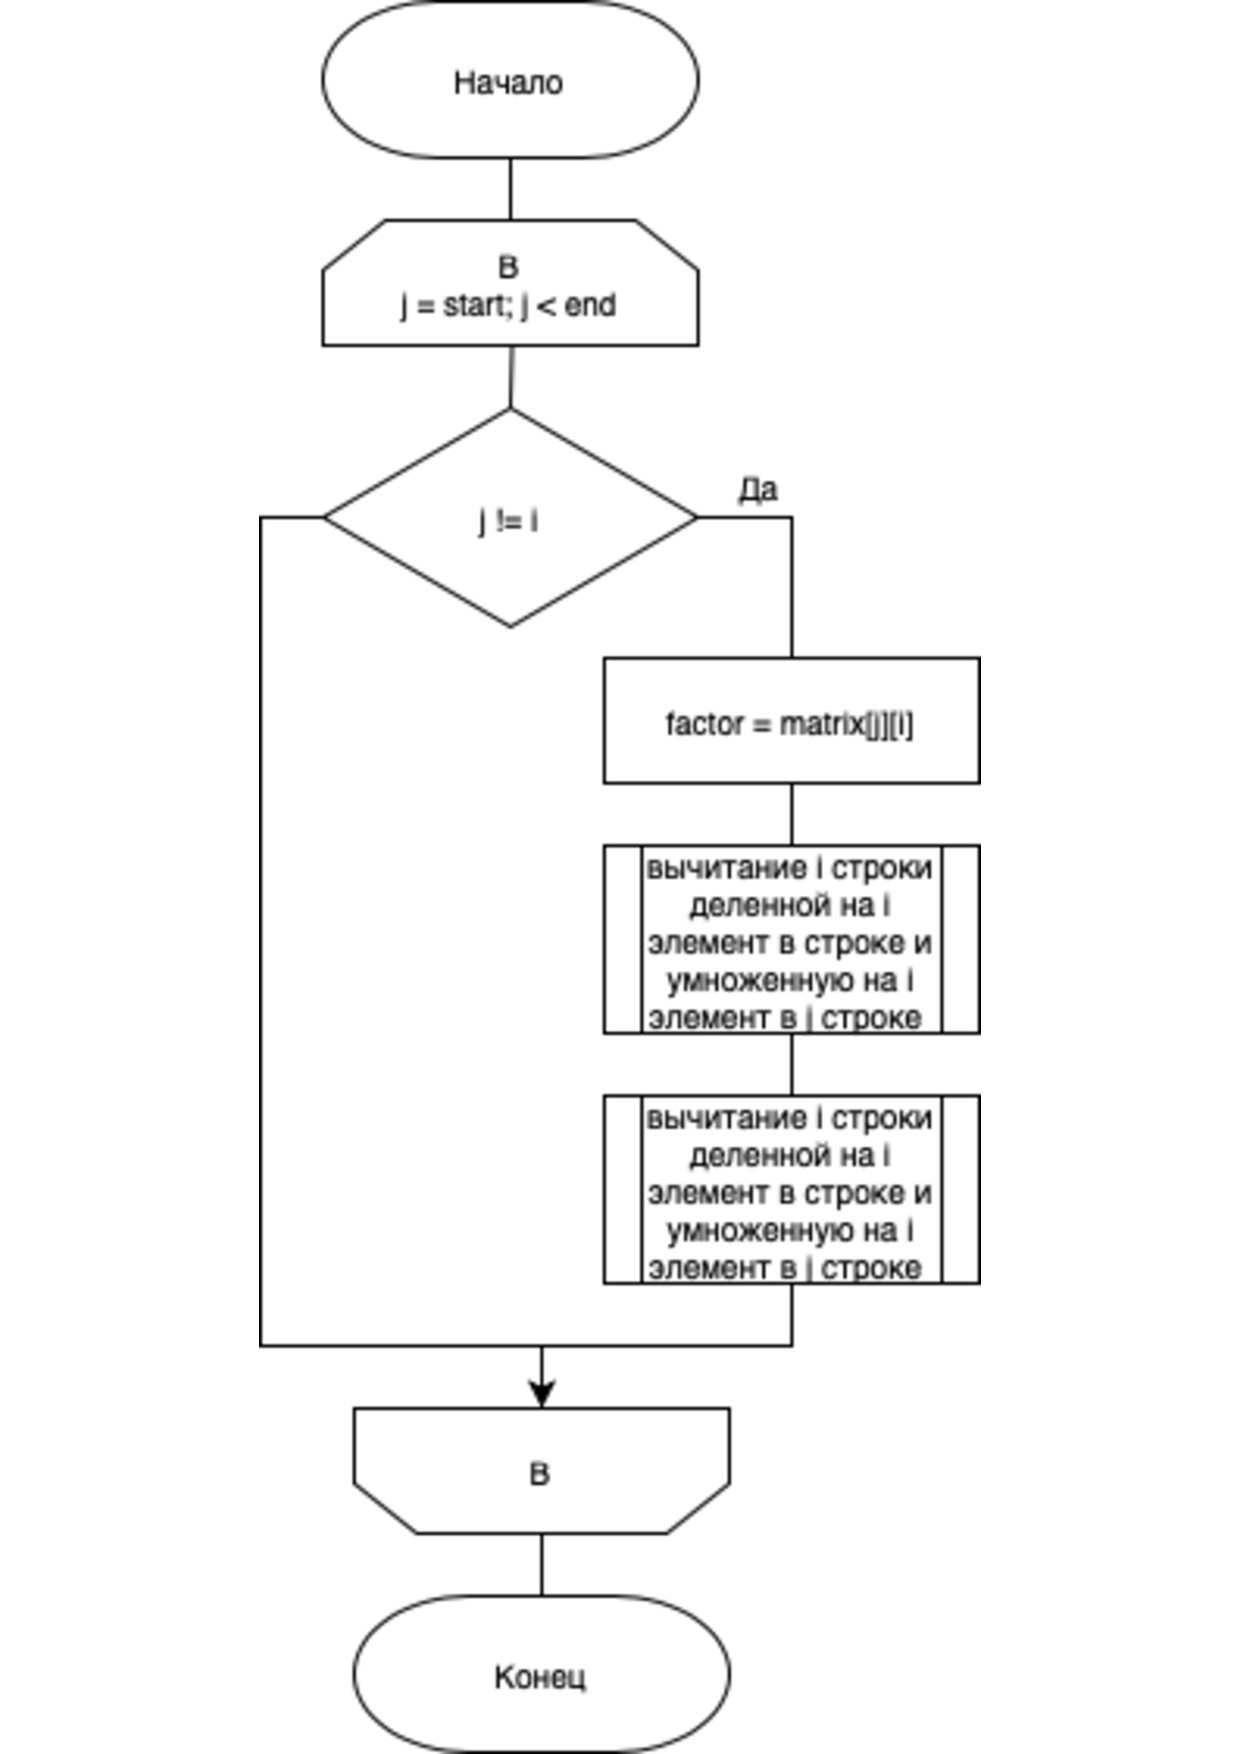
\includegraphics[width=0.7\linewidth]{img/paral5.pdf}
    \caption{Схема параллельного алгоритма вычитания из строк матрицы модифицированной текущей строки}
    \label{fig:paral5}
\end{figure}

\clearpage
\section{Структура разрабатываемого программного обеспечения}

Для реализации разрабатываемого программного обеспечения будет использоваться
метод структурного программирования. Каждый из алгоритмов будет представлен
отдельной функцией, при необходимости будут выделены подпрограммы для каждой из
них. Также будут реализованы функции для ввода-вывода матрицы, функции для
выделения памяти.

\section*{Вывод}
На основе теоретических данных, полученных из аналитического раздела, 
были построены схемы для алгоритмов метода Гаусса-Жордана и параллельной реализации.
